\documentclass[12pt,letterpaper]{report}

\usepackage[utf8]{inputenc}
\usepackage[T1]{fontenc}
\usepackage[spanish,es-noindentfirst]{babel}
\usepackage[margin=2.5cm]{geometry}
\usepackage{hyperref}
\usepackage{enumitem}
\usepackage{amsmath}
\usepackage{graphicx}
\usepackage{titlesec}
\usepackage{xcolor}
\usepackage{booktabs}
\usepackage{float}
\usepackage{array}

\addto\captionsspanish{\renewcommand{\tablename}{Tabla}}

\hypersetup{
    colorlinks=true,
    linkcolor=black,
    citecolor=black,
    urlcolor=blue,
    pdftitle={Bitácora Co-MIL - Parte IV},
    pdfauthor={Adrián Emiliano Beltrán Fernández}
}

% Estilo de entrada de bitácora fechada, consistente con las Partes I--III.
\newcommand{\entrada}[2]{%
    \vspace{0.6em}
    \noindent\textbf{#1.} \textit{#2}
    \vspace{0.3em}
    \par
}

\title{\textbf{Bitácora de Investigación y Diseño Arquitectónico \\ Co-MIL --- Parte IV \\[0.3em]
\large Reformulación metodológica y estudio de eficiencia de anotación}}
\author{Adrián Emiliano Beltrán Fernández \\ \small Estudiante de Física Biomédica \\ \small Facultad de Ciencias, UNAM \\[1em]
\small Tutor: Dr.\ José Eduardo Chairez Veloz \\ \small Profesor de Asignatura B, Facultad de Ciencias, UNAM}
\date{Ciudad de México, 2026 \\ \small Documento vivo --- última actualización: 2 de septiembre de 2026}

\begin{document}

\maketitle

\begin{abstract}
\noindent Esta parte continúa el registro cronológico iniciado en \texttt{co\_mil\_bitacora.pdf}
(Parte I), \texttt{co\_mil\_bitacora\_parte2.pdf} (Parte II) y \texttt{co\_mil\_bitacora\_parte3.pdf}
(Parte III). Documenta el \textbf{cambio de estrategia} acordado en la reunión con el tutor y la
asesoría clínica del 27 de agosto de 2026 --- pasar de anotación débil por cajas a \textbf{anotación
densa (máscaras de tejido)} --- y el trabajo de la primera semana de septiembre: una investigación
dirigida de estado del arte verificada fuente por fuente, el reencuadre del proyecto en tres brazos
de supervisión, y un primer estudio computacional sobre el conjunto de datos público DFUTissue que
establece un baseline supervisado y un resultado preliminar sobre \emph{cuántas máscaras densas hacen
falta} para localizar tejidos. El catálogo de tejidos y el protocolo de anotación quedan como
propuesta a confirmar en la sesión con la Escuela Nacional de Enfermería y Obstetricia (ENEO)
programada para la semana del 8 de septiembre.
\end{abstract}

\tableofcontents

\chapter{Reformulación tras la reunión del 27 de agosto de 2026}

\section{27 de agosto de 2026}

\entrada{Reunión de seguimiento con el tutor y la asesoría clínica}{Asistieron el Dr.\ José Eduardo
Chairez Veloz (tutor) y el Dr.\ Gerardo, el especialista clínico que participó en la anotación de las
primeras imágenes del lote. Reunión de carácter informal, apoyada en una presentación visual de 11
diapositivas publicada como página web.}

El tutor planteó un cambio de fondo en la estrategia de anotación, motivado por el hallazgo de
atención plana documentado en la Parte III (mediana de contraste de atención $\approx 0.04$ en escala
0--1, con el 97.8\,\% de las bolsas de prueba conteniendo un solo tipo de tejido). Las decisiones y
observaciones de la reunión:

\begin{itemize}[leftmargin=1.5em]
    \item \textbf{Anotación densa desde ahora.} Se abandona la anotación por cajas delimitadoras
        (\texttt{generador\_bolsas.py}) y se adopta la anotación por \emph{contorno de cada tejido}
        (polígonos, máscara a nivel de píxel), al estilo del artículo previo del grupo. De una
        anotación densa se derivan de forma automática y consistente todas las versiones más simples
        (etiqueta por imagen, máscara binaria tejido/no-tejido); al revés no es posible.
    \item \textbf{Herramienta: MATLAB Image Labeler} (versión web). Funciona en cualquier equipo con
        navegador --- incluidos los que no usan Windows, resolviendo la incompatibilidad que impidió
        al Dr.\ Gerardo colaborar de forma remota hasta ahora --- y tanto el tutor como el autor
        cuentan con licencia. Integra asistencia por \emph{Segment Anything Model} (SAM) para
        acelerar el trazado.
    \item \textbf{Catálogo reducido.} No las 12 clases del catálogo actual, sino solo las de mayor
        relevancia clínica y que los modelos distinguen mejor. La cantidad y elección exactas quedan
        para acordar con la asesoría clínica.
    \item \textbf{Clasificación binaria.} Además de la multiclase, una tarea binaria tejido/no-tejido,
        equivalente a la máscara de herida del artículo previo. Es el resultado más robusto
        estadísticamente con un conjunto de datos pequeño.
    \item \textbf{Confusión sobre el mallado ``estilo CAM''.} El Dr.\ observó que la malla de
        instancias del prototipo CAM (Parte III) era mucho más fina que la de los parches recortados
        a mano y le pareció adecuada. Aclaración registrada: esa finura proviene de los campos
        receptivos de la red convolucional (la rejilla nativa del mapa de características, $\sim$32
        veces menor que la entrada), no de la anotación; un mapa puede verse detallado y ser
        incorrecto --- de hecho la primera corrida del rediseño CAM dio AUC-ROC $\leq 0.5$ en
        clasificación.
    \item \textbf{Colaboración con enfermería.} El tutor gestionó el apoyo de la Escuela Nacional de
        Enfermería y Obstetricia (ENEO) de la UNAM. Sesión programada para la semana del 8 de
        septiembre: las especialistas en tejidos capacitan al equipo en su identificación clínica; el
        equipo del proyecto explica el protocolo de anotación digital.
\end{itemize}

\section{2 de septiembre de 2026}

\entrada{Investigación dirigida de estado del arte, verificada fuente por fuente}{Antes de comprometer
la nueva estrategia se realizó una revisión dirigida sobre tres preguntas concretas, con cada cita
comprobada de forma independiente contra la fuente primaria (arXiv, PubMed, sitios de editoriales).
Notas completas archivadas en el material de proceso del autor.}

\begin{itemize}[leftmargin=1.5em]
    \item \textbf{Localización de tejidos con supervisión débil o parcial.} A la escala de datos de
        este proyecto (decenas a un par de centenas de imágenes) y con máscaras densas disponibles,
        el estado del arte para localizar es la \emph{segmentación semántica supervisada ligera}
        (decodificador FPN o U-Net sobre un extractor MobileNetV2). El Aprendizaje Multi-Instancia
        (MIL) no es la herramienta de localización cuando hay máscaras --- es lo que se usa cuando
        solo hay etiqueta de imagen. Precedente casi idéntico: Kabir \emph{et al.} (2025,
        arXiv:2502.10652) segmentan 6 tejidos en 147 fotografías macroscópicas de heridas y obtienen
        Dice $\approx 0.82$ con FPN. Advertencia relevante: los métodos MIL recientes contra el
        colapso de atención (AEM, MICCAI 2025; ASMIL, 2026) atacan el problema \emph{opuesto}
        (atención demasiado concentrada en laminillas de patología); aplicarlos aquí aplanaría aún
        más los mapas.
    \item \textbf{Aprendizaje continuo.} El nicho de MIL con aprendizaje continuo tiene apenas cuatro
        o cinco trabajos, todos sobre laminillas completas de patología salvo uno (Ebrahimi
        \emph{et al.}, MICCAI-W 2025, células de sangre). Un estudio cuidadoso de \emph{rehearsal}
        (búfer de repetición) es una contribución legítima, no una reimplementación. Li \emph{et al.}
        (CVPR 2025) reportan que en MIL con atención el olvido catastrófico se concentra en las capas
        de atención.
    \item \textbf{Conjuntos de datos y huecos del campo.} Solo existen dos conjuntos de datos de
        \emph{tejidos} de herida disponibles públicamente en el mundo: DFUTissue (110 imágenes, 3
        clases) y WoundTissue (147 imágenes, 6 clases). Las revisiones recientes (Yu \emph{et al.},
        \emph{Digital Health} 2026 --- que cita el trabajo previo del grupo; Reifs Jiménez
        \emph{et al.}, \emph{J.\ Med.\ Syst.} 2025) señalan como carencias explícitas: conjuntos de
        datos pequeños y homogéneos, poca diversidad de tono de piel, localización menos desarrollada
        que clasificación, y falta de rigor en la generación del ground truth. \textbf{Ningún trabajo
        de heridas ha publicado una curva de eficiencia de anotación, y no existe ningún estudio de
        aprendizaje continuo en el dominio.}
\end{itemize}

\entrada{El proyecto reformulado: de ``MIL lo es todo'' a ``MIL es un brazo''}{Reencuadre acordado a
partir de la investigación anterior.}

En la Parte III todo el sistema era un modelo MIL con atención, y la localización espacial se
esperaba de sus mapas de atención --- que resultaron casi planos. Con anotación densa, la
localización deja de depender de la atención: se resuelve como segmentación supervisada. El MIL se
conserva, pero como el \emph{instrumento} de las variantes de anotación barata, no como el sistema
completo. La Figura~\ref{fig:reformulado} resume la estructura.

\begin{figure}[H]
\centering
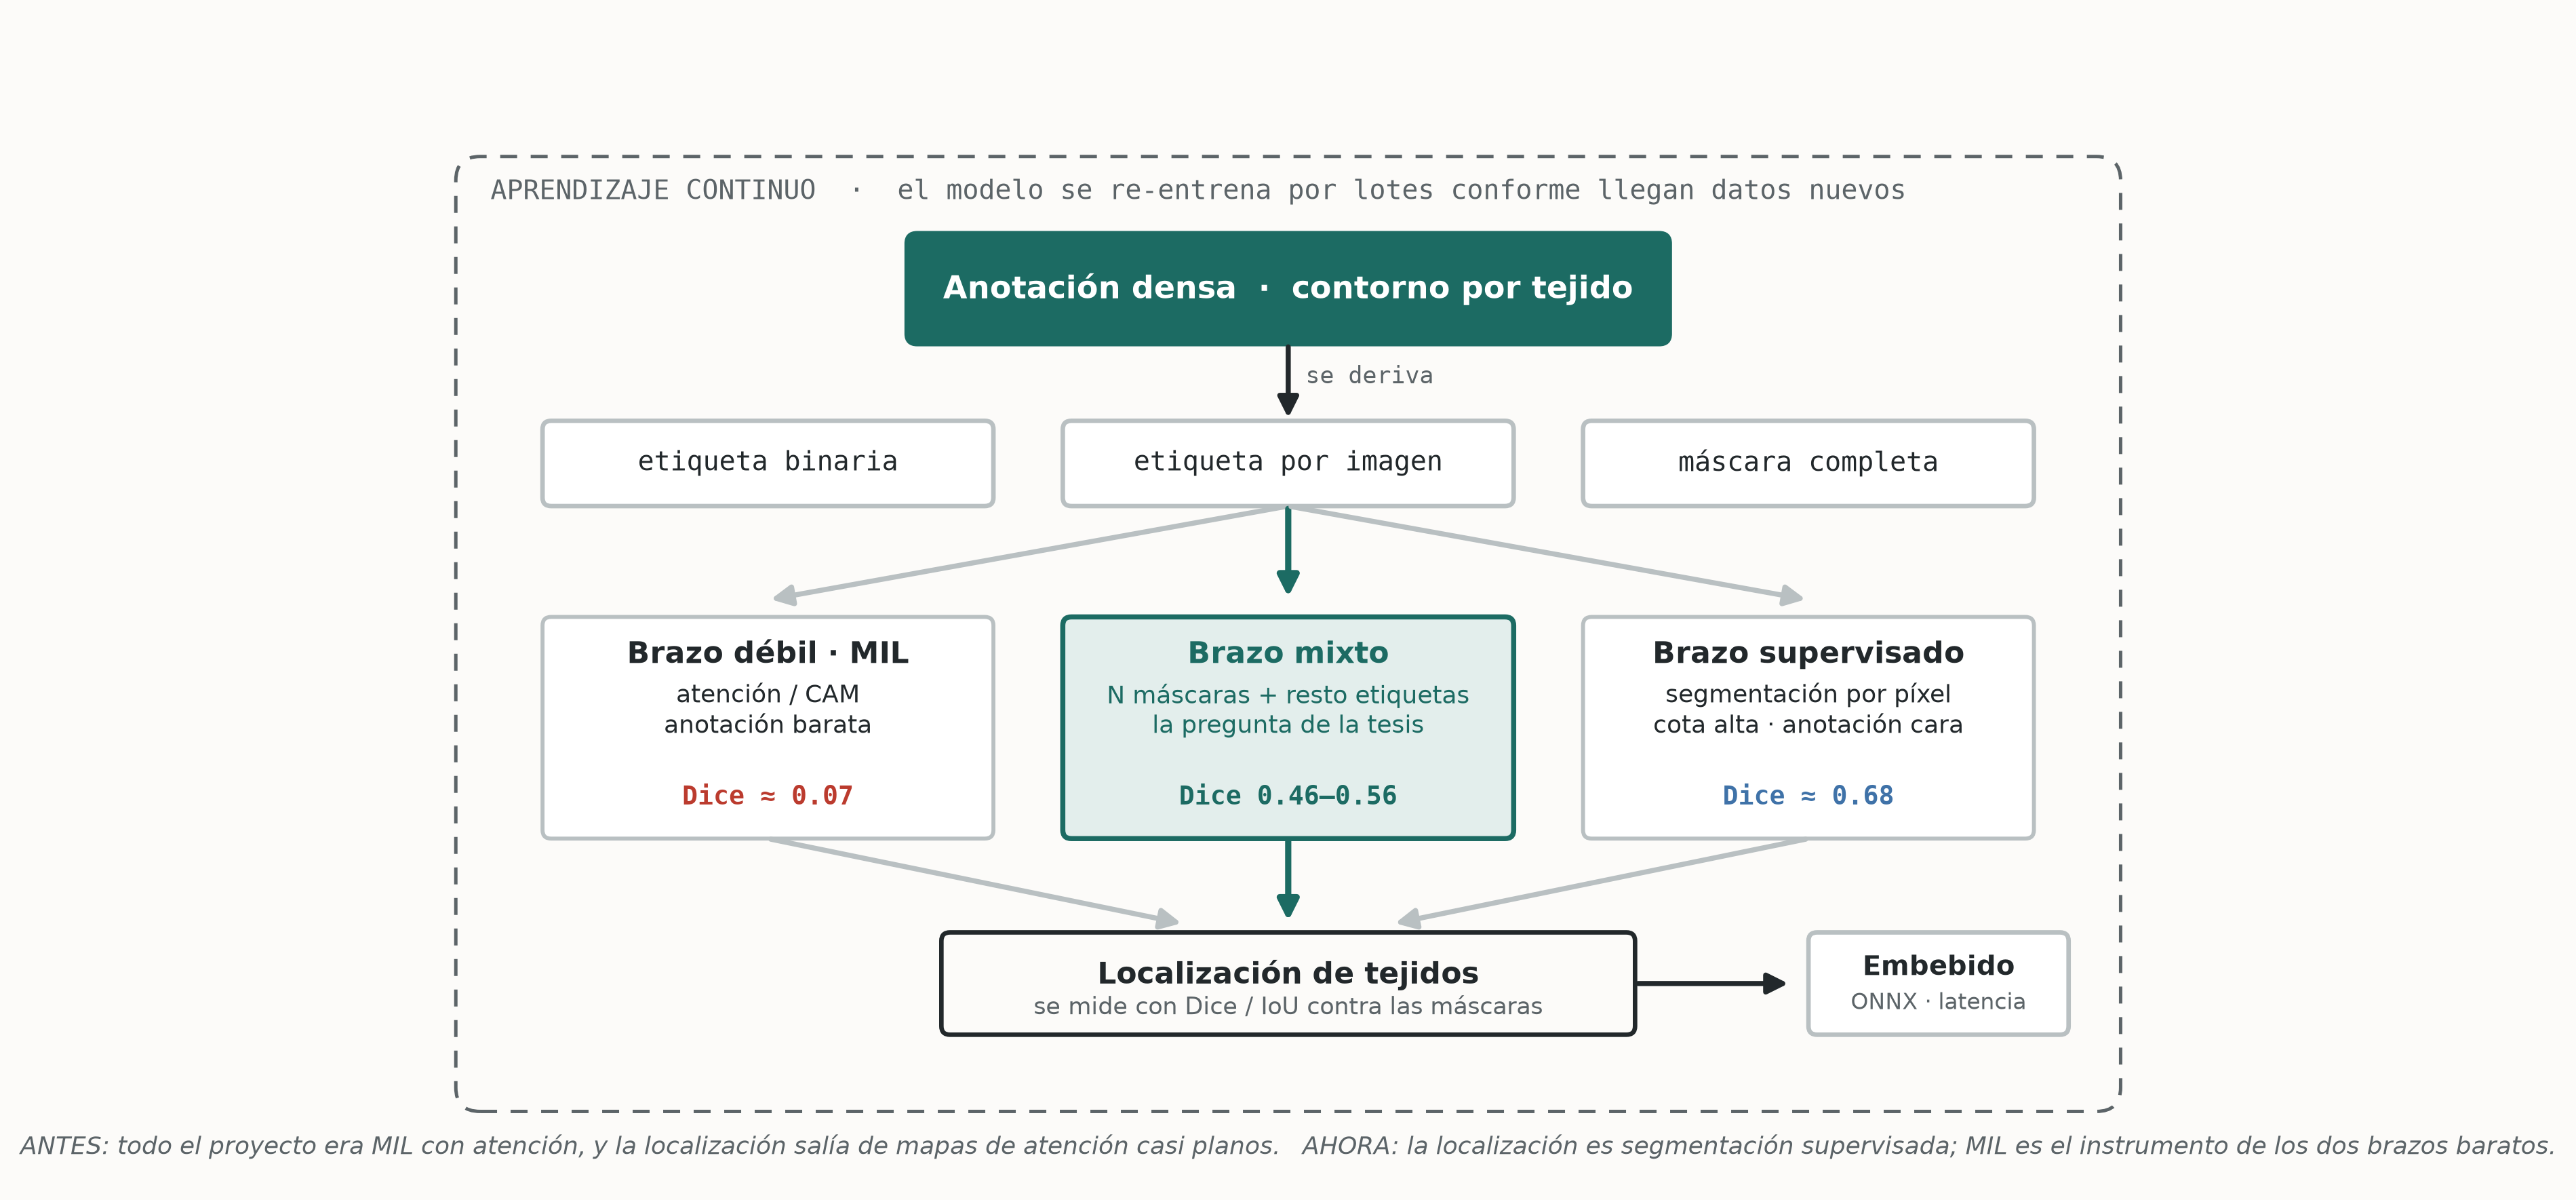
\includegraphics[width=\textwidth]{figuras/fig_proyecto_reformulado.png}
\caption{El proyecto reformulado. De una única anotación densa se derivan tres niveles de etiqueta;
tres brazos de entrenamiento las consumen; los tres se evalúan de forma idéntica, contra las
máscaras. El brazo mixto (pocas máscaras + muchas etiquetas débiles) es la pregunta central. Encima,
el aprendizaje continuo re-entrena el modelo conforme llegan lotes de datos; al final se exporta a un
dispositivo de bajo consumo.}
\label{fig:reformulado}
\end{figure}

La estructura de la tesis queda en seis componentes, alineados con los objetivos del plan y con tres
ejes de contribución que no han sido abordados en heridas: (1)~un conjunto de datos regional mexicano
con diversidad de tono de piel; (2)~la frontera de eficiencia de anotación; (3)~el aprendizaje
continuo.

\begin{enumerate}[leftmargin=1.6em]
    \item \textbf{Conjunto de datos} mexicano (5 clases, multi-anotador) + validación de transferencia
        entre poblaciones con DFUTissue en las 3 clases compartidas.
    \item \textbf{Brazo supervisado}: segmentación semántica ligera (FPN + MobileNetV2). La cota alta.
    \item \textbf{Brazo débil (MIL)}: solo etiqueta de imagen. ¿Hasta dónde llega?
    \item \textbf{Brazo mixto}: pocas máscaras densas + muchas etiquetas débiles. La curva Dice
        frente a número de máscaras.
    \item \textbf{Extensión de aprendizaje continuo}: datos que llegan por lotes; olvido y
        \emph{rehearsal}.
    \item \textbf{Factibilidad embebida}: exportación a ONNX, latencia, compromiso multi-tejido vs.\
        binaria.
\end{enumerate}

\entrada{Catálogo de tejidos propuesto (5 clases)}{Propuesta fundamentada, a confirmar en la sesión
con la ENEO. Detalle completo en \texttt{documentación/propuesta\_dataset\_tejidos\_UPD.pdf}.}

Se propone anotar cinco categorías, elegidas por relevancia clínica para la cicatrización, evidencia
en la literatura de que los modelos las distinguen, y prevalencia esperada suficiente
(Figura~\ref{fig:cinco}):

\begin{enumerate}[leftmargin=1.6em]
    \item \textbf{Granulación} (rojo) --- tejido que cicatriza; la clase mejor distinguida en toda la
        literatura (Dice típico 0.70--0.91).
    \item \textbf{Fibrina / esfacelo} (amarillo) --- frena la cicatrización; el tejido del lecho más
        difícil (Dice 0.33--0.77 según el trabajo).
    \item \textbf{Tejido calloso} (hiperqueratosis) --- propio del pie diabético; ya presente en el
        trabajo previo y en DFUTissue.
    \item \textbf{Tejido necrótico / escara} (negro) --- indica desbridamiento; alto contraste visual.
    \item \textbf{Piel perilesional} (intacta o macerada) --- presente en \emph{todas} las
        fotografías, lo que equilibra el conjunto y define directamente la máscara binaria.
\end{enumerate}

Las tres primeras coinciden con DFUTissue y con el artículo previo, lo que habilita la validación
cruzada entre poblaciones. Se dejan fuera hueso y tendón expuestos (prevalencia demasiado baja para
aprenderlos: 0 y 1 de 204 bolsas en el lote actual) e hiperpigmentación (se confunde con el tono de
piel del paciente y puede introducir sesgo). La clasificación binaria tejido/no-tejido sale sola del
esquema: el lecho (clases 1--4) es ``tejido''; la piel perilesional y el fondo son ``no tejido''.

\begin{figure}[H]
\centering
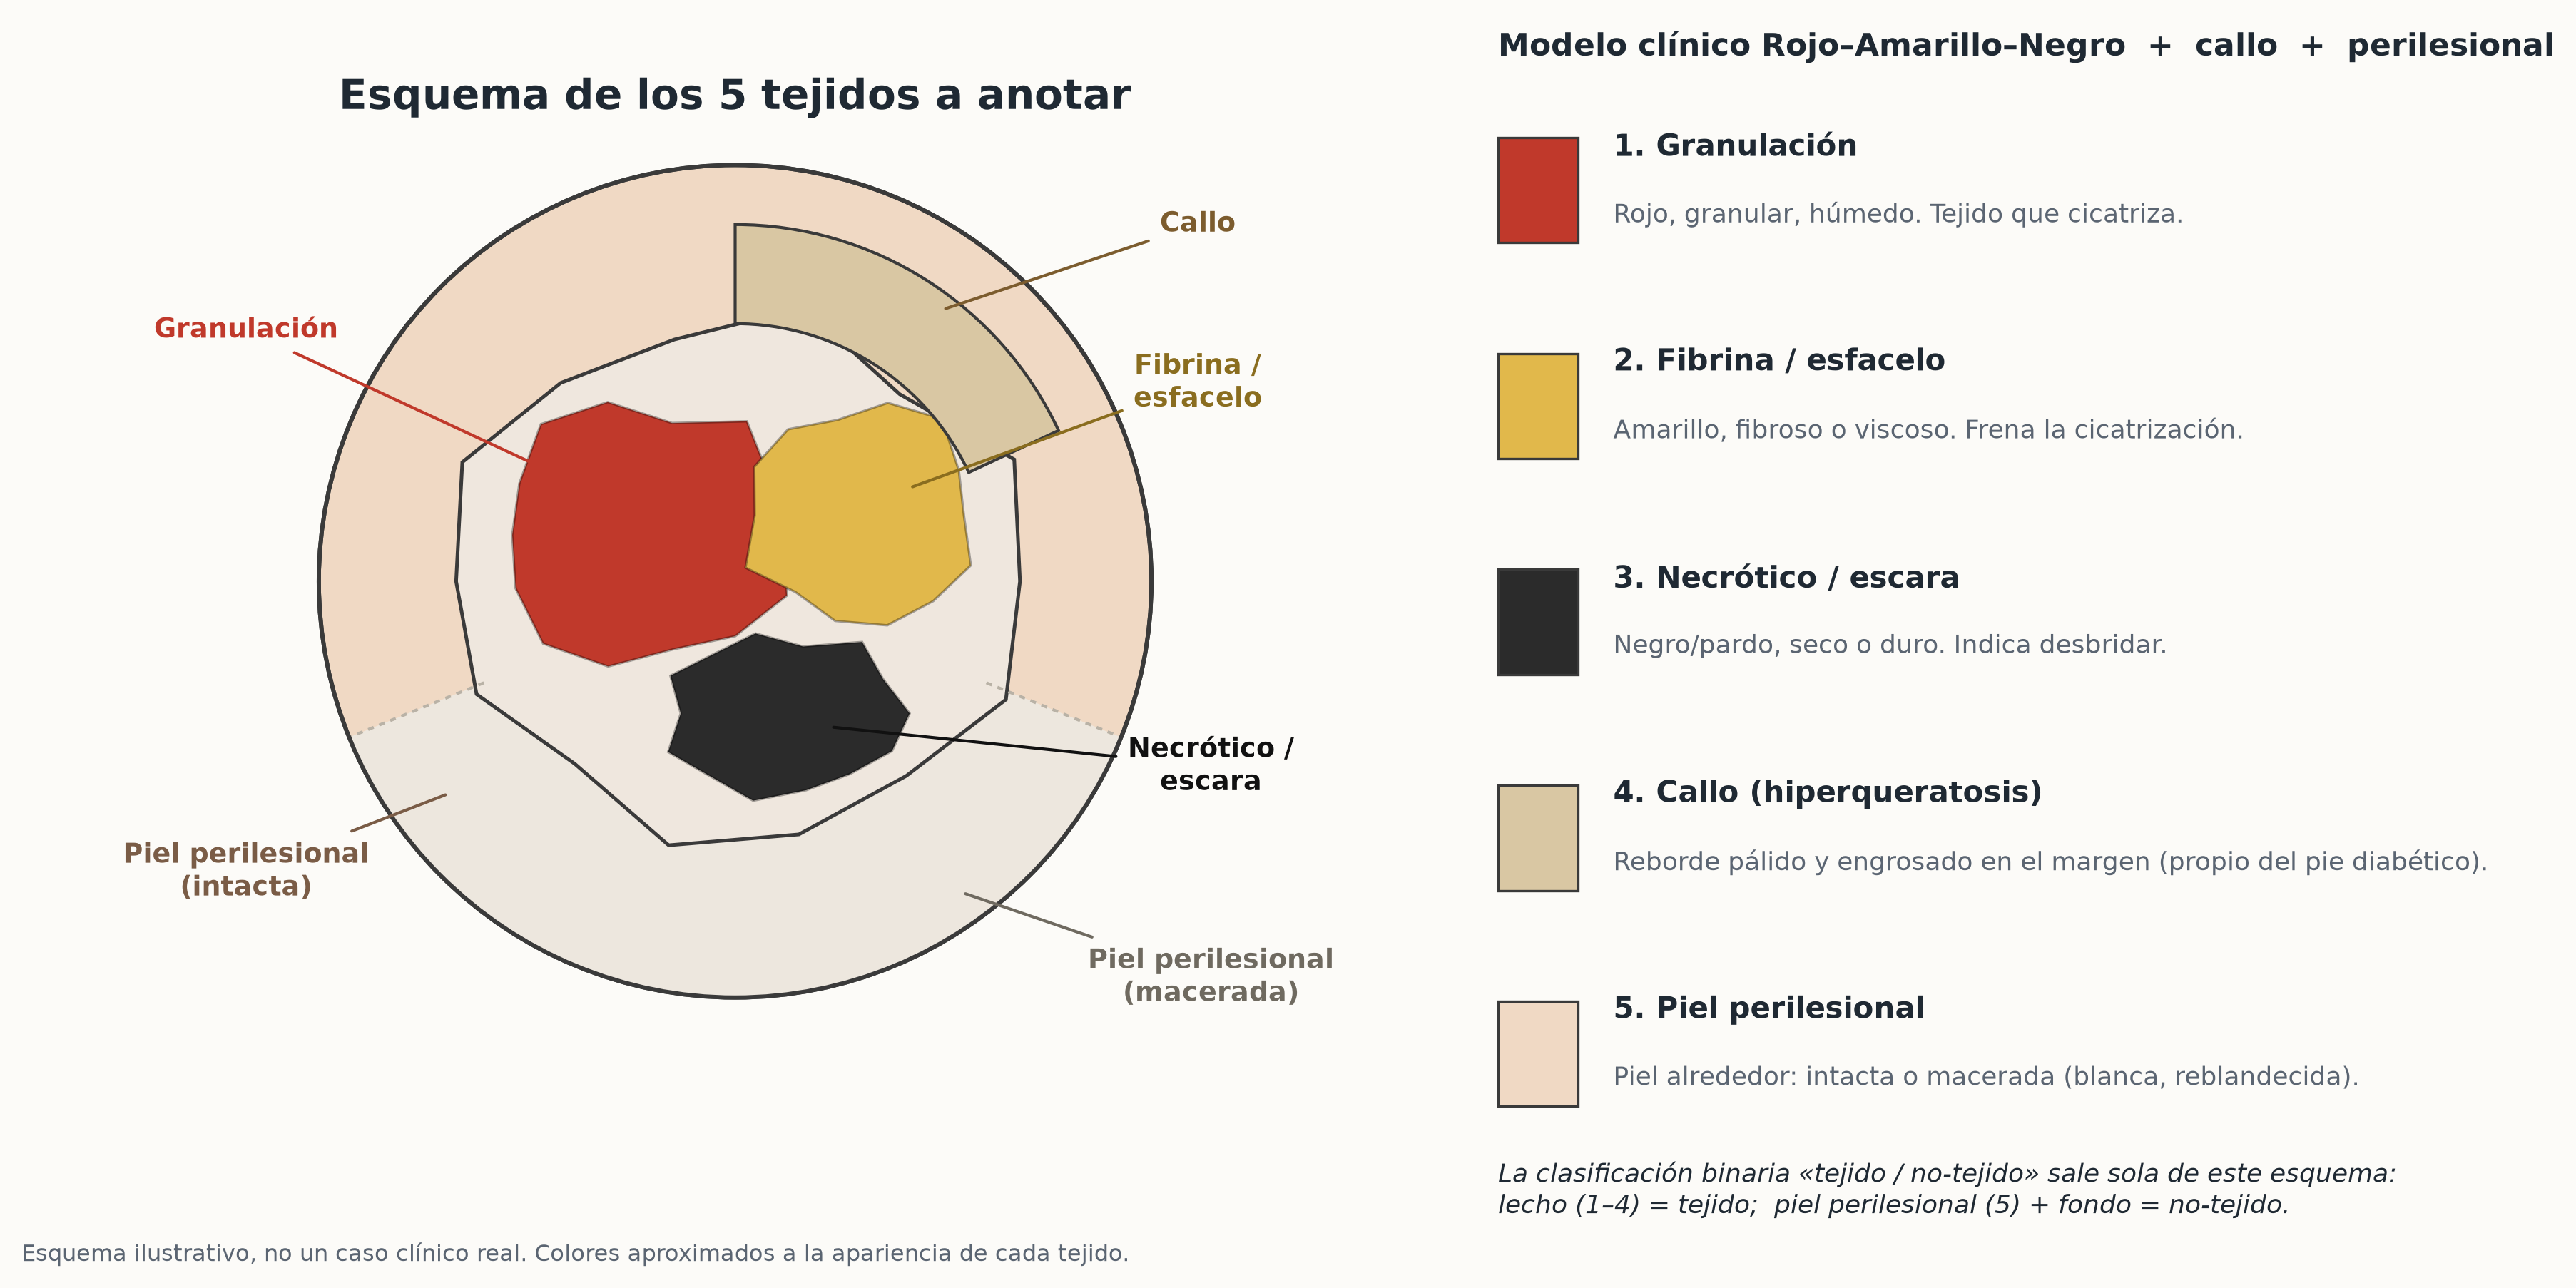
\includegraphics[width=\textwidth]{figuras/fig_esquema_5_tejidos.png}
\caption{Las cinco categorías propuestas, sobre el modelo clínico Rojo--Amarillo--Negro ampliado con
callo y piel perilesional. Esquema ilustrativo, no un caso clínico real.}
\label{fig:cinco}
\end{figure}

\entrada{Reconciliación con el artículo previo del grupo}{Se revisó el texto completo de
Maldonado-Oclica \emph{et al.} (2025), del que el autor es coautor, para fijar la vara de medir con
precisión.}

Corrección respecto a lo que se había registrado: la segmentación de tejido de ese trabajo
\textbf{sí} se hizo con aprendizaje profundo (ensamble de ResUnet + Unet++), no con \emph{k-means} ---
el \emph{k-means} de color era un análisis aparte. Los resultados reportados (sobre DFUTissue, con
partición 70:15:15) y los del baseline propio de esta semana (T2, sección siguiente, partición
oficial 78:16:16):

\begin{table}[H]
\centering
\caption{Dice por tejido en DFUTissue. ``Italia'' = Maldonado-Oclica \emph{et al.}\ (2025); ``T2'' =
baseline de esta bitácora (FPN + MobileNetV2, 4.2\,M de parámetros, CPU). Los conjuntos de prueba no
son idénticos, así que la comparación es indicativa.}
\begin{tabular}{lrrr}
\toprule
Tejido & Italia (ResUnet+Unet++) & T2 (FPN+MobileNetV2) & Diferencia \\
\midrule
Fibrina     & 0.333 & 0.455 & $+0.122$ \\
Granulación & 0.786 & 0.874 & $+0.088$ \\
Callo       & 0.515 & 0.712 & $+0.197$ \\
\midrule
Media       & 0.545 & 0.680 & $+0.135$ \\
\bottomrule
\end{tabular}
\end{table}

Un modelo ligero, sin optimizar, entrenado en CPU, ya supera al trabajo previo en las tres clases.
\textbf{Superar sus cifras es alcanzable y no es el reto principal}; se hará como resultado
secundario, con una arquitectura y una receta de entrenamiento mejores. La contribución fuerte de la
tesis son los tres ejes ya mencionados, no ganar por unas décimas de Dice.

\section{Trabajo computacional sobre datos públicos (DFUTissue)}

Mientras avanza la anotación --- que es el camino crítico y depende de terceros --- el trabajo de
modelado se adelanta sobre conjuntos de datos públicos. El código nuevo vive en
\texttt{CO-MIL/segmentacion/} y no reemplaza nada del pipeline MIL original.

\entrada{T1 --- conjuntos de datos públicos}{Descarga reproducible con el script
\texttt{descargar\_datos.py} del módulo nuevo.}

\textbf{DFUTissue} (Dhar \emph{et al.}, 2024, arXiv:2406.16012): 110 imágenes de úlcera de pie
diabético anotadas por píxel para tres tejidos (fibrina, granulación, callo) más fondo, con partición
oficial 78/16/16 y un conjunto adicional de 600 imágenes sin etiquetar. Son regiones de interés
recortadas y rellenadas a $256\times256$\,px. El repositorio no declara licencia formal; el uso se
condiciona a citar el artículo. \textbf{WoundTissue} (Kabir \emph{et al.}, 2025): el repositorio
público contiene solo 13 imágenes de muestra --- el conjunto completo (147 imágenes, 6 tejidos, con
licencia CC BY-NC-SA 4.0) se solicita a los autores por correo.

\entrada{T2 --- baseline supervisado}{\texttt{CO-MIL/segmentacion/entrenar\_seg.py}.}

Se entrenó un modelo \textbf{FPN con extractor MobileNetV2} (4.2\,M de parámetros, pensado para
despliegue embebido), preentrenado en ImageNet, con pérdida Dice + entropía cruzada, sobre las 78
imágenes de entrenamiento de DFUTissue; 122 épocas, $\sim$46\,min en CPU. La
Figura~\ref{fig:arquitectura} detalla la arquitectura, incluyendo la segunda cabeza de supervisión
débil que se usa en el brazo mixto (T3/T4). Resultado sobre las 16 imágenes de prueba oficiales:

\begin{figure}[H]
\centering
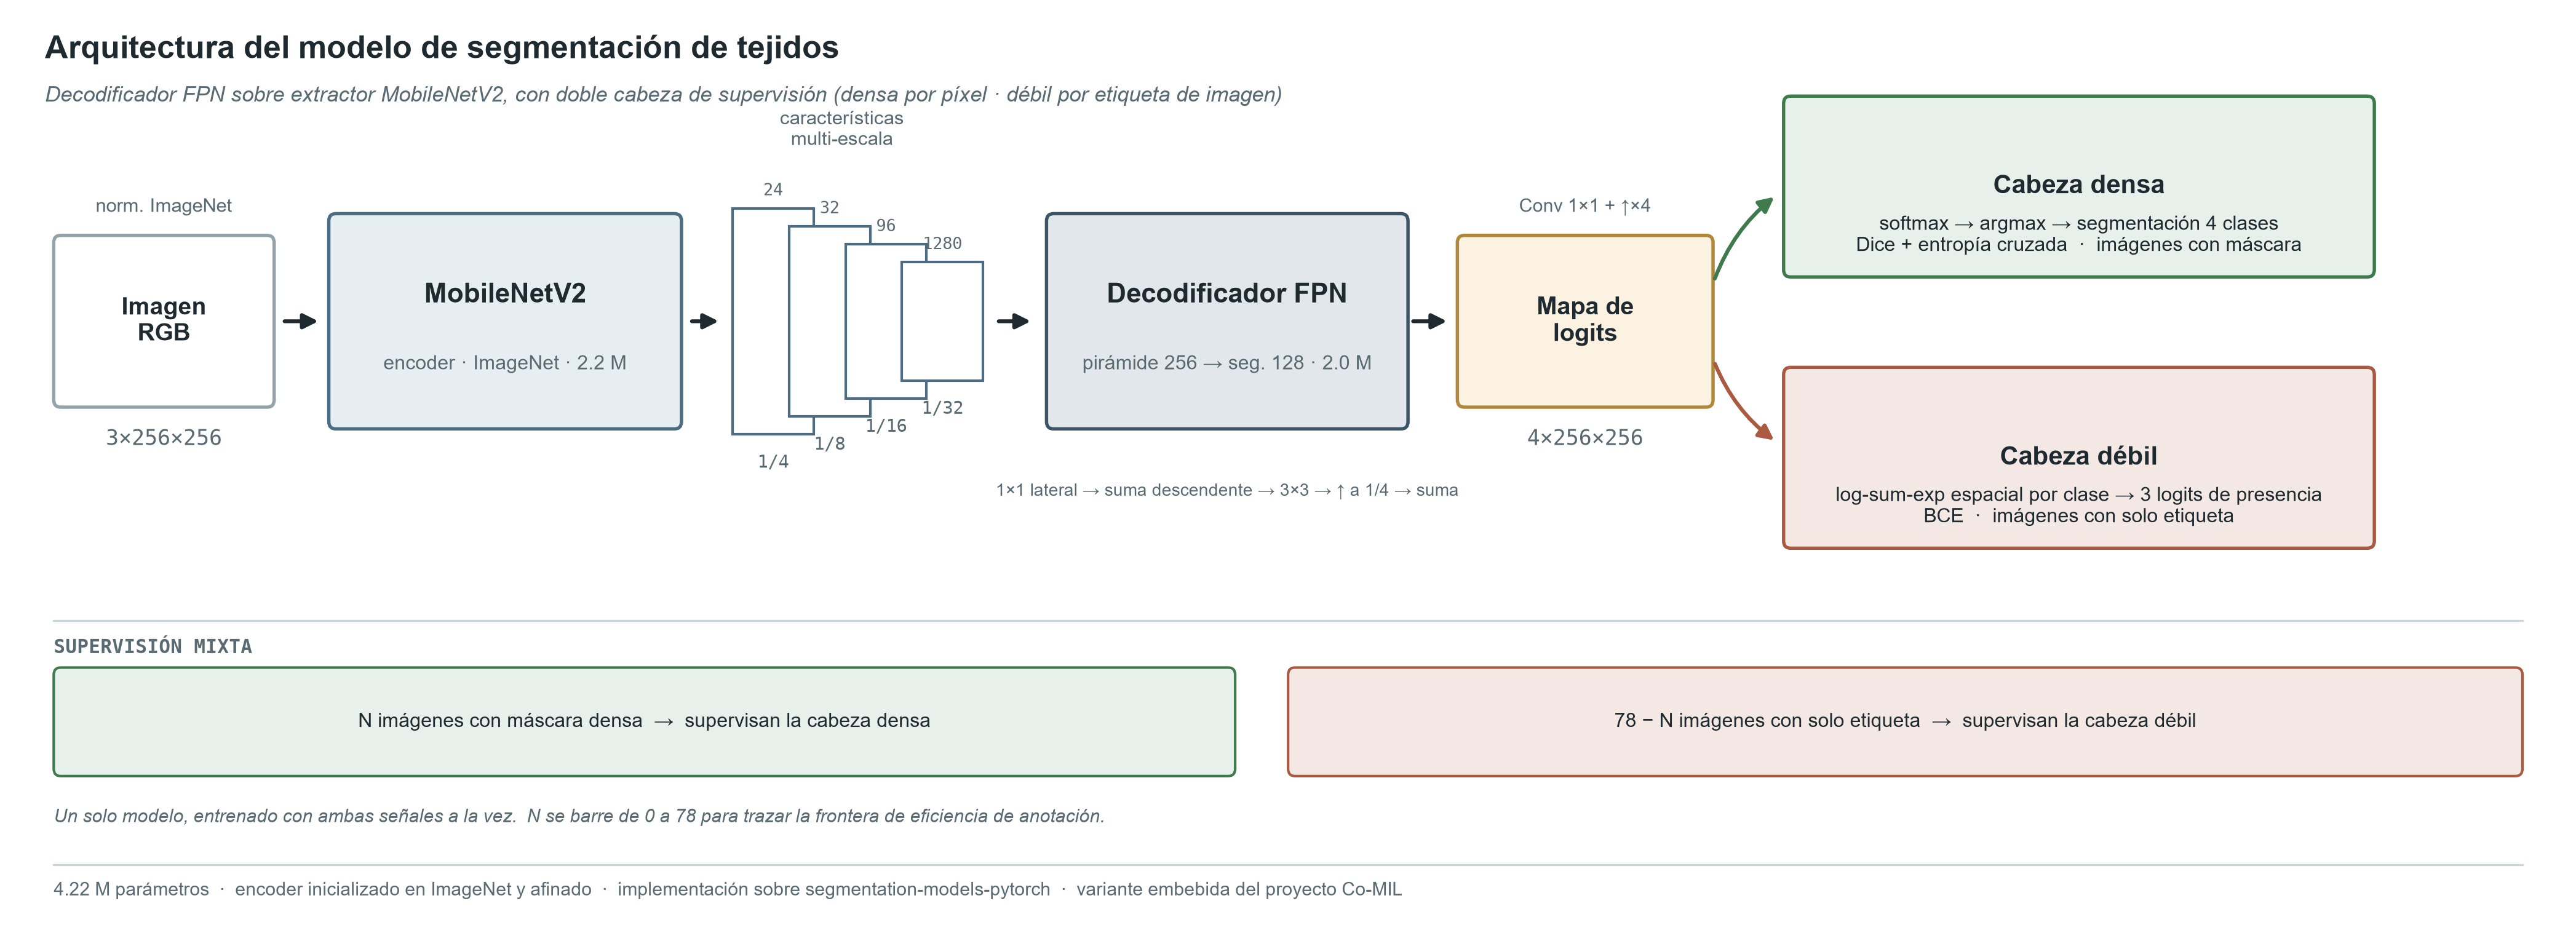
\includegraphics[width=\textwidth]{figuras/fig_arquitectura_segmentacion.png}
\caption{Arquitectura del modelo de segmentación de tejidos. El extractor MobileNetV2 (inicializado
en ImageNet) produce características a cuatro escalas; el decodificador FPN las fusiona y genera un
mapa de logits de $4\times256\times256$. De ese mapa parten dos cabezas: la \emph{densa} (softmax +
argmax, con pérdida Dice + entropía cruzada frente a la máscara) y la \emph{débil} (agrupación
log-sum-exp por clase, con entropía cruzada binaria frente a la etiqueta de imagen). Un único modelo
se entrena con ambas señales: las $N$ imágenes con máscara supervisan la cabeza densa y las $78-N$
con solo etiqueta, la débil.}
\label{fig:arquitectura}
\end{figure}

\begin{table}[H]
\centering
\caption{T2 --- Dice e IoU por clase, split de prueba de DFUTissue.}
\begin{tabular}{lrr}
\toprule
Clase & Dice & IoU \\
\midrule
Granulación & 0.874 & 0.775 \\
Tejido calloso & 0.712 & 0.553 \\
Fibrina & 0.455 & 0.295 \\
\midrule
Media (tejidos) & 0.680 & 0.541 \\
\bottomrule
\end{tabular}
\end{table}

Interpretación: baseline sano y en el rango de la literatura. La fibrina es el eslabón débil, como en
todos los trabajos del área. El techo de referencia en DFUTissue es su propio artículo (Unet + MiT-b3,
un modelo $\sim$10 veces más pesado): Dice medio $\approx 0.85$.

\entrada{T3 y T4 --- supervisión débil y frontera de eficiencia de anotación}{%
\texttt{CO-MIL/segmentacion/entrenar\_eficiencia.py}. Responde a la pregunta central del brazo mixto.}

\textbf{Mecanismo} (Figura~\ref{fig:mixta}). Un único modelo FPN + MobileNetV2 se entrena con una
mezcla: $N$ imágenes con máscara densa (pérdida de segmentación, comparación píxel a píxel) y las
$78-N$ restantes con solo la etiqueta de qué tejidos contienen. Para estas últimas se agrupa el mapa
de logits de cada clase con \emph{log-sum-exp} en un único valor y se compara con la etiqueta
mediante entropía cruzada binaria --- el mecanismo estándar de segmentación débilmente supervisada:
enseña ``hay / no hay este tejido'', no dónde. Se barre $N \in \{0, 5, 10, 20, 40, 78\}$: $N=0$ es
supervisión puramente débil (T3); $N=78$ es supervisión densa completa; la curva Dice frente a $N$ es
la frontera de eficiencia (T4). La evaluación es idéntica en todos los puntos, para que la
comparación aísle solo el efecto de la cantidad de anotación densa.

\begin{figure}[H]
\centering
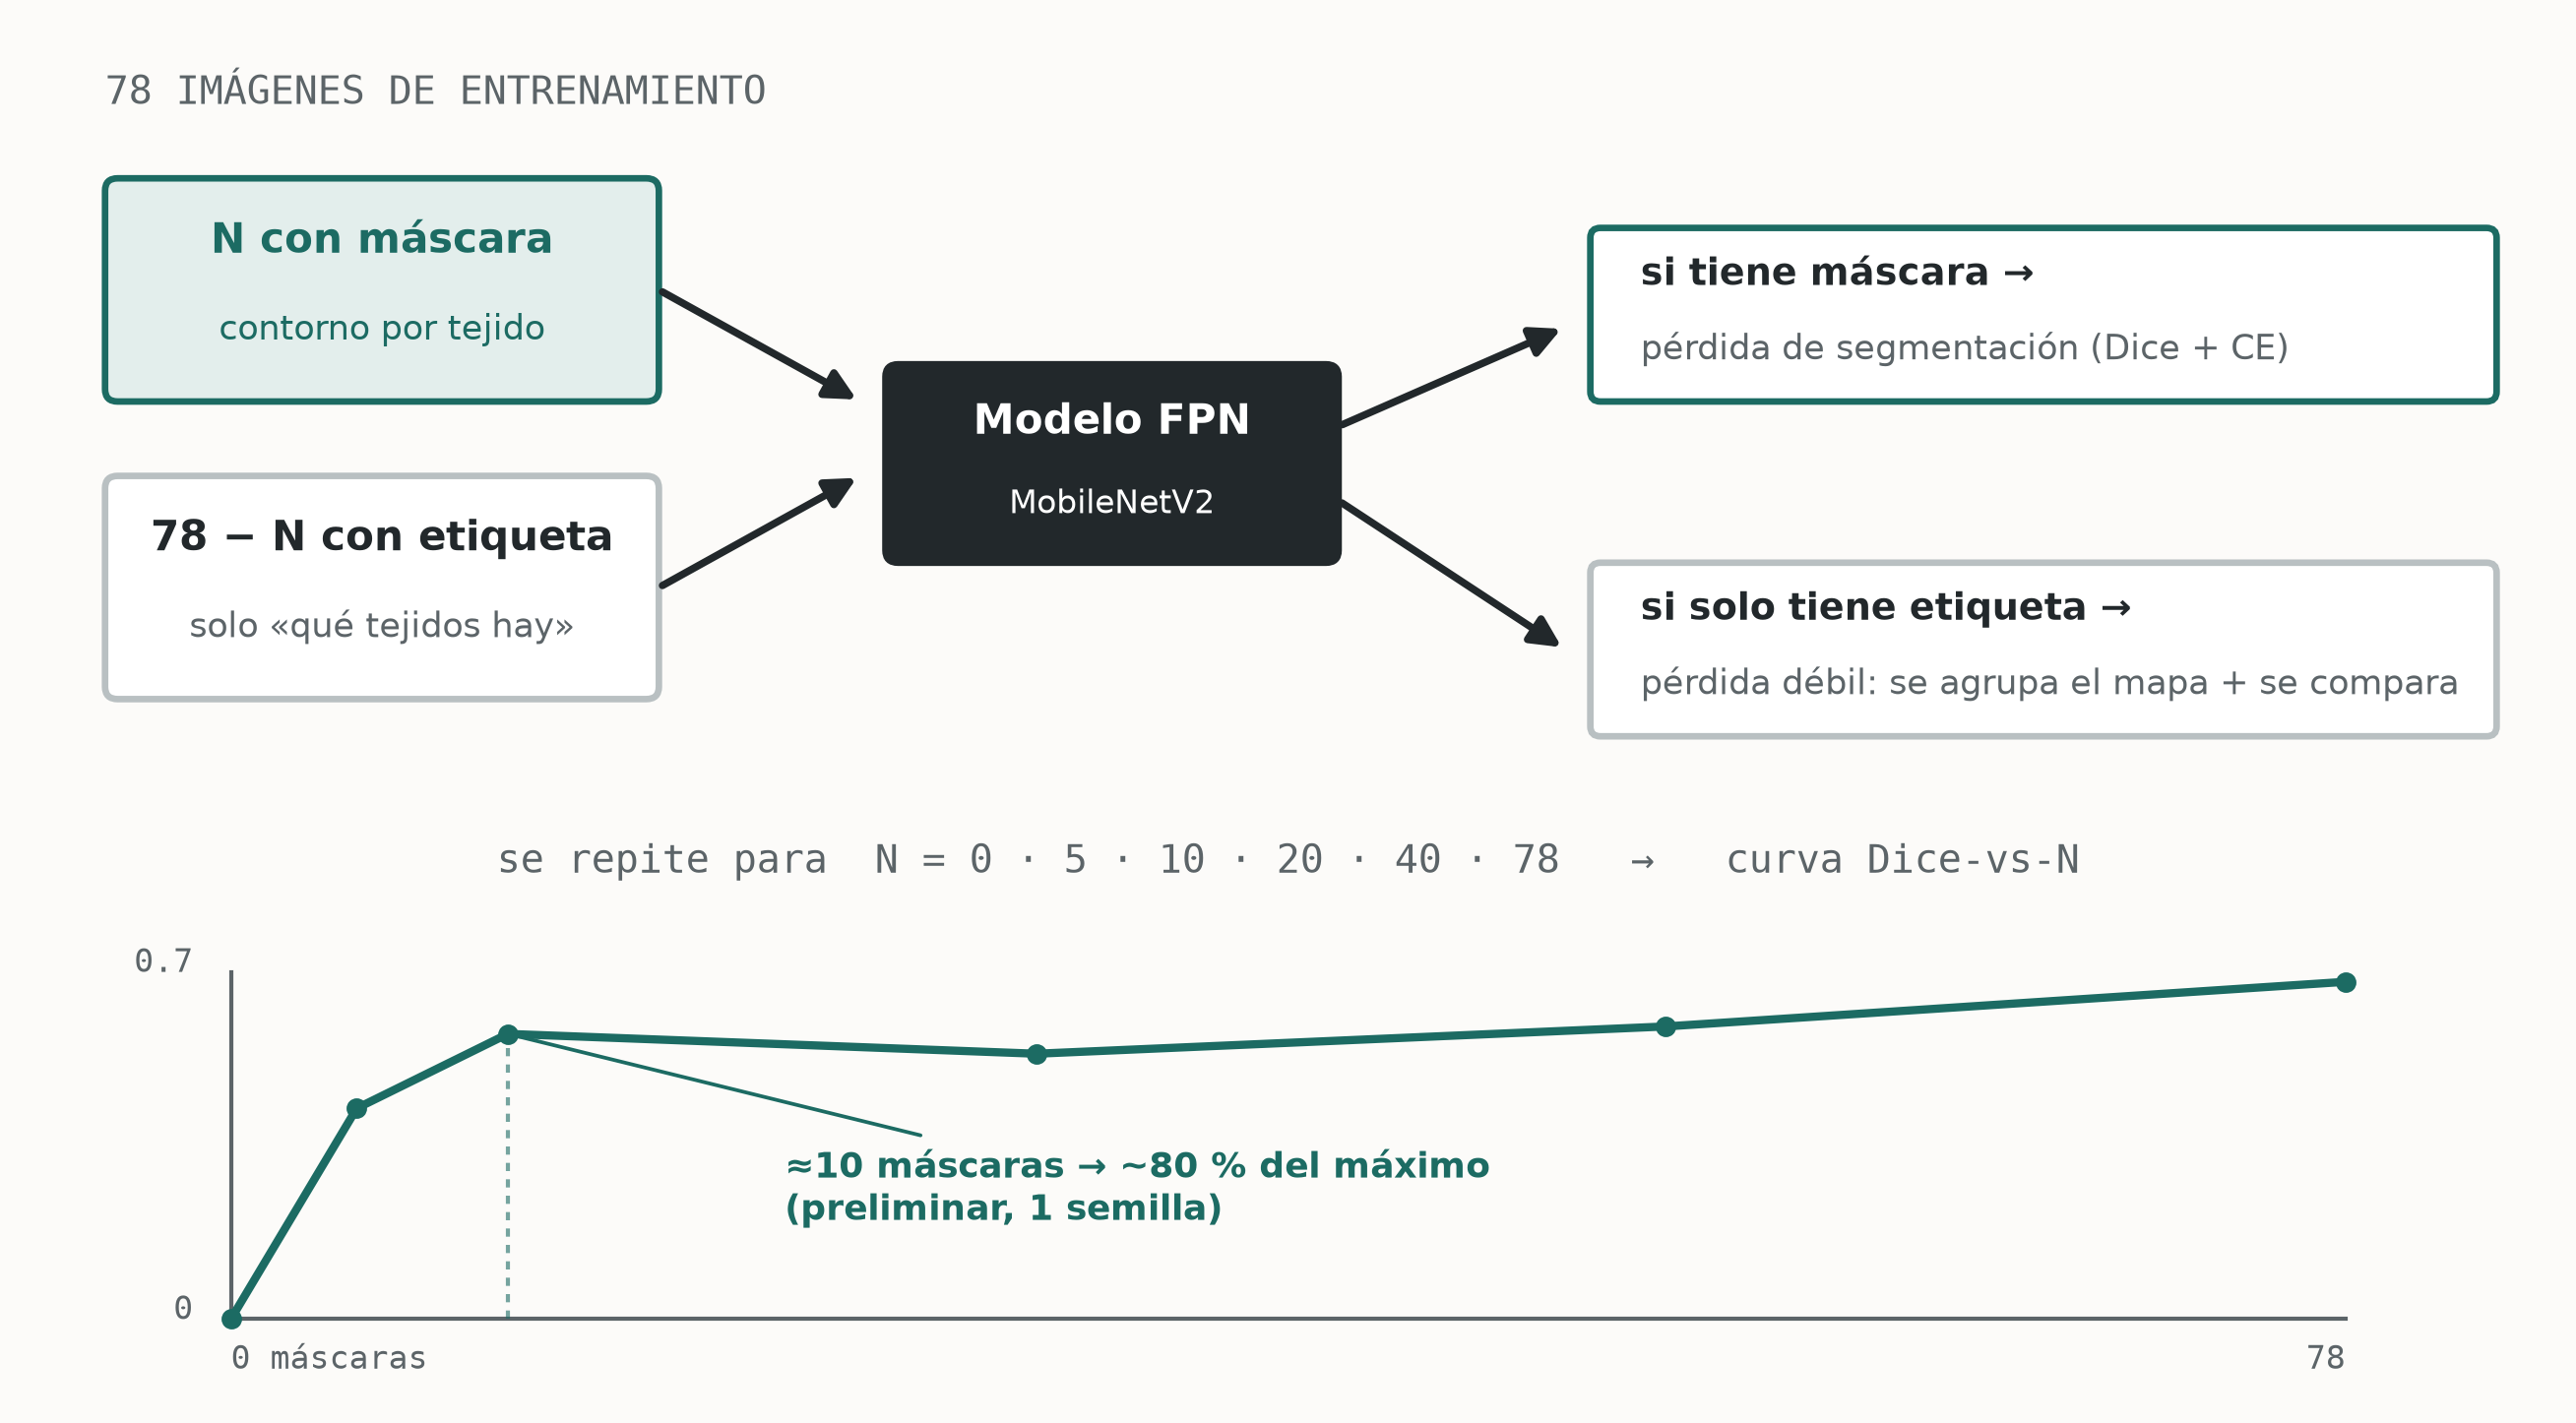
\includegraphics[width=\textwidth]{figuras/fig_supervision_mixta.png}
\caption{El mecanismo de supervisión mixta. Un modelo aprende de dos señales a la vez; el barrido de
$N$ produce la curva de eficiencia. La curva mostrada es esquemática.}
\label{fig:mixta}
\end{figure}

\textbf{Resultado preliminar} (una sola semilla, Figura~\ref{fig:curva}):

\begin{table}[H]
\centering
\caption{T3/T4 preliminar --- Dice en el split de prueba de DFUTissue, según el número de máscaras
densas. $N=0$: solo etiqueta de imagen. $N=78$: supervisión densa completa.}
\begin{tabular}{rrrrr}
\toprule
$N$ & Fibrina & Granulación & Callo & Media \\
\midrule
0  & 0.00 & 0.00 & 0.20 & 0.07 \\
5  & 0.07 & 0.76 & 0.56 & 0.46 \\
10 & 0.30 & 0.81 & 0.55 & 0.55 \\
20 & 0.21 & 0.73 & 0.59 & 0.51 \\
40 & 0.24 & 0.84 & 0.61 & 0.56 \\
78 & 0.50 & 0.88 & 0.71 & 0.70 \\
\bottomrule
\end{tabular}
\end{table}

\begin{figure}[H]
\centering
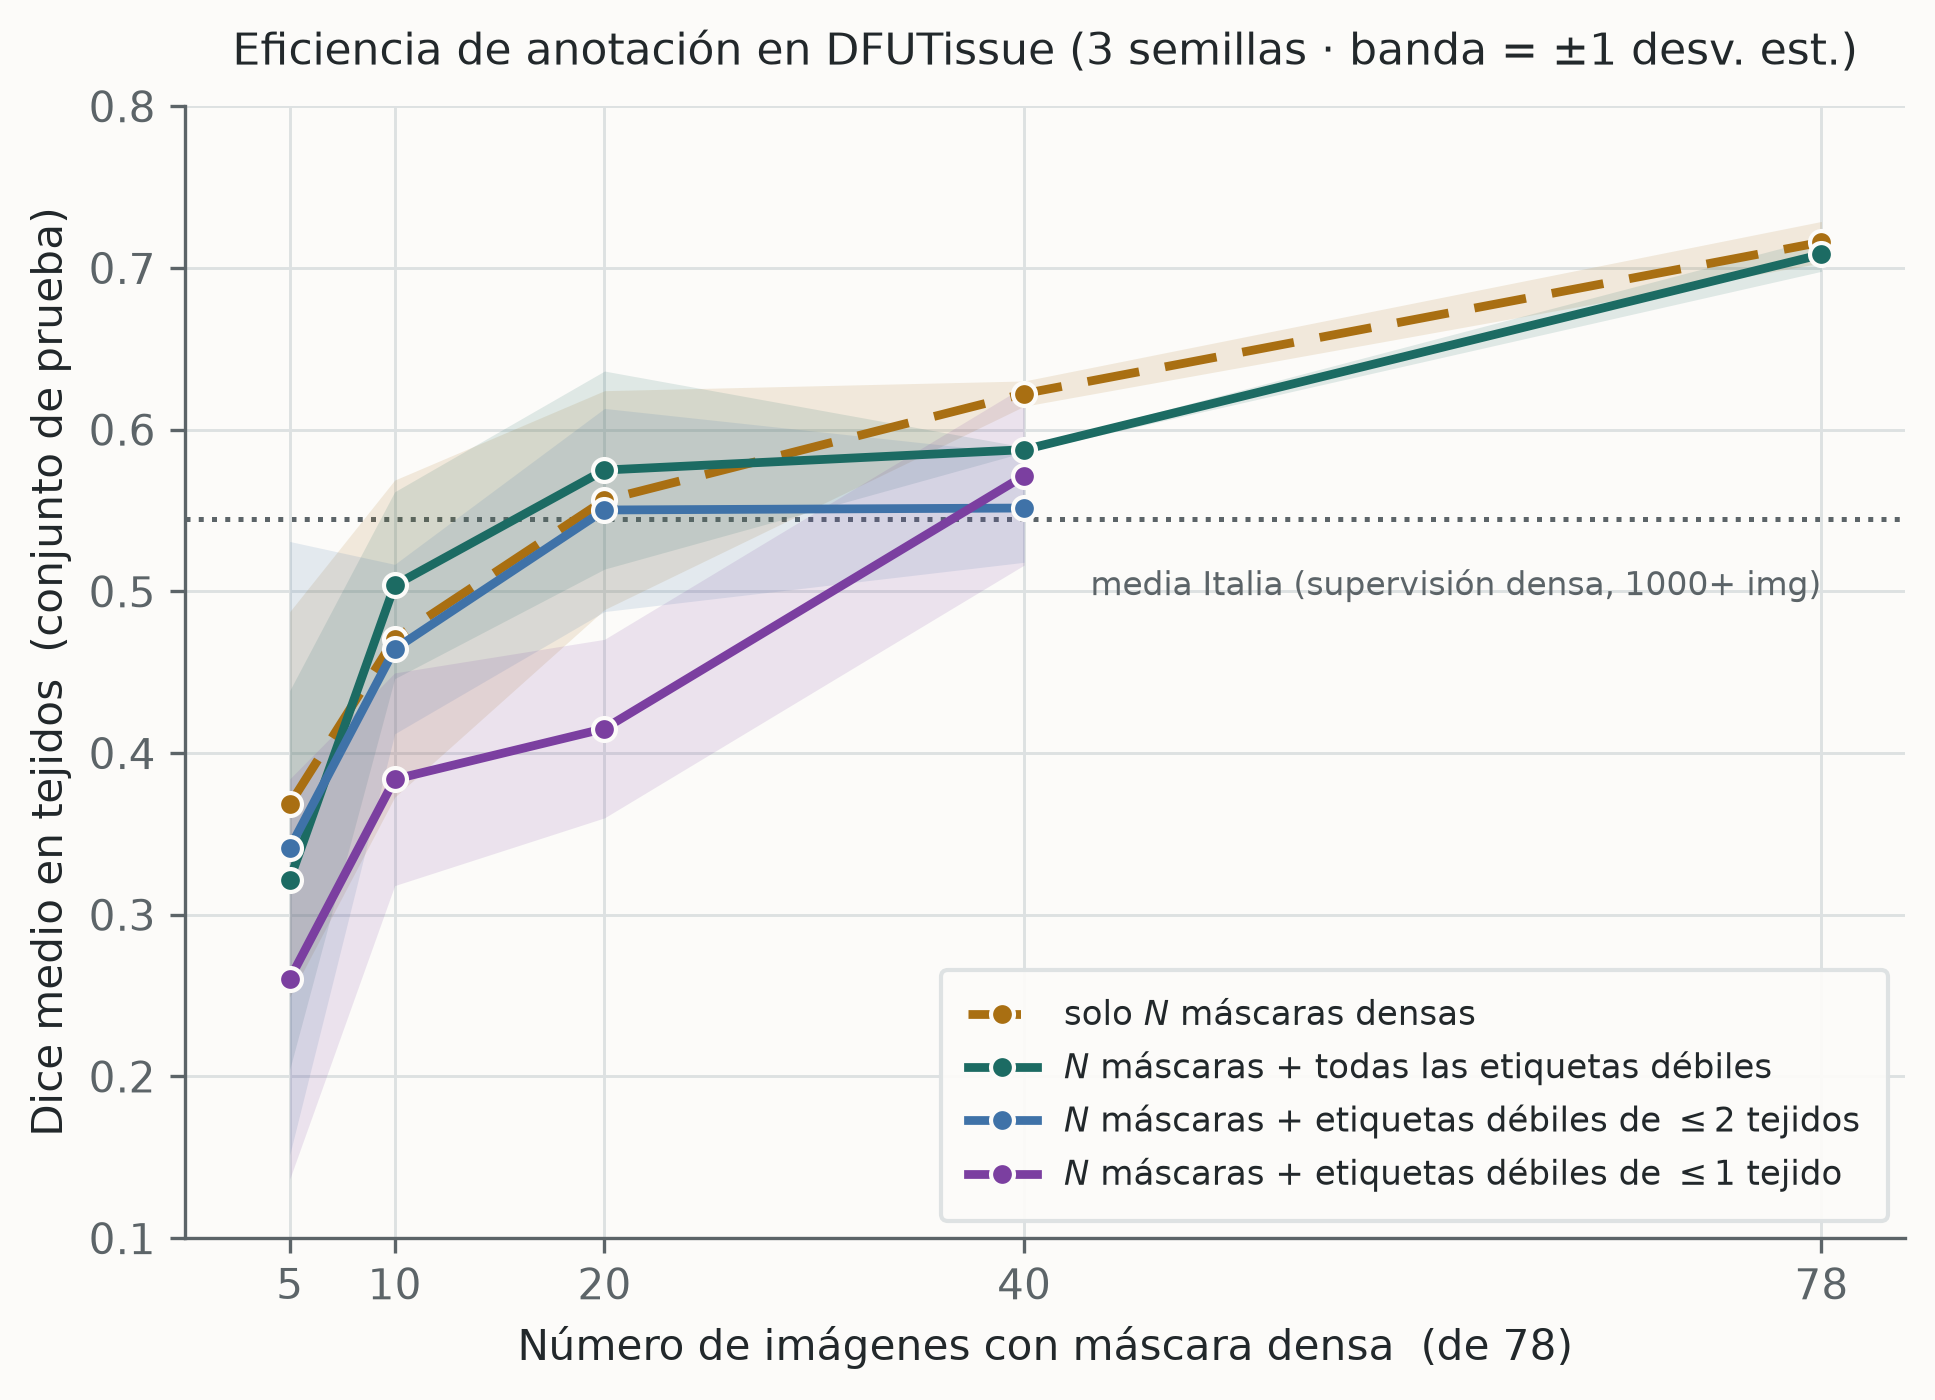
\includegraphics[width=0.92\textwidth]{figuras/fig_curva_eficiencia_dfutissue.png}
\caption{Frontera de eficiencia de anotación en DFUTissue (resultado preliminar, una semilla).}
\label{fig:curva}
\end{figure}

\textbf{Lecturas y cautelas:}
\begin{itemize}[leftmargin=1.5em]
    \item Con supervisión puramente débil ($N=0$) el modelo no localiza (Dice 0.07). Coincide con la
        literatura: los métodos de segmentación débilmente supervisada necesitan miles de imágenes
        para converger.
    \item Con $\sim$10 máscaras densas (13\,\% de las imágenes) se recupera $\sim$80\,\% del
        desempeño de la supervisión densa completa. La curva sube casi vertical hasta $N \approx 10$
        y luego se aplana.
    \item La fibrina es la única clase que sigue mejorando con más máscaras densas; granulación y
        callo saturan pronto.
    \item \textbf{Pendiente crítico:} la curva anterior siempre tiene supervisión débil en las
        imágenes sin máscara. Falta el control ``$N$ máscaras y nada más'', para saber si la
        anotación débil \emph{aporta algo} o si es solo el modelo aprendiendo de $N$ muestras. El
        experimento está preparado (\texttt{--modos mixto,solo\_supervisado}) y se corre en GPU
        (Google Colab) con tres semillas y bandas de error, junto con una receta de entrenamiento
        reforzada (aumentación fuerte, pérdida Tversky, sobre-muestreo de la clase rara) y una
        comparación de arquitecturas (Unet++, SegFormer). El notebook es
        \texttt{CO-MIL/segmentacion/colab\_estudio\_dfutissue.ipynb}.
    \item El bache no monótono entre $N=10$ y $N=20$ es ruido de una sola semilla --- con un conjunto
        pequeño, qué imágenes caen en el subconjunto ``con máscara'' influye mucho.
\end{itemize}

\section{Plan de trabajo y estado}

\entrada{Camino crítico y trabajo en paralelo}{Registro para no repetir la discusión.}

\begin{itemize}[leftmargin=1.5em]
    \item La \textbf{anotación densa} es el camino crítico y no depende por completo del autor
        (participan la ENEO y el Dr.\ Gerardo). Estimación realista: semanas a un par de meses para
        60--150 imágenes con asistencia y SAM.
    \item \textbf{En paralelo, desde ya}, sobre datos públicos: baselines de segmentación (hecho, T2),
        el estudio de eficiencia con varias semillas y la ablación de supervisión débil (en curso, en
        GPU), un prototipo de aprendizaje continuo, y la factibilidad embebida. Todo esto ya es
        material de capítulos.
    \item \textbf{Bloqueado hasta la sesión con la ENEO} (semana del 8 de septiembre): fijar el
        catálogo de 5 clases y los criterios de anotación; a partir de ahí, la versión definitiva del
        protocolo y la reescritura de la hoja de ruta.
    \item Si el componente de aprendizaje continuo resulta demasiado ruidoso con el tamaño de datos
        disponible, se presenta como diseño completo + resultados parciales + trabajo futuro, y aun
        así la tesis se sostiene sobre el conjunto de datos, la eficiencia de anotación y la
        factibilidad embebida.
\end{itemize}

\entrada{Diagramas y material visual}{Estado del material figurativo tras el pivote.}

Figuras ya generadas para esta parte y para la propuesta clínica, todas versionadas en
\texttt{documentación/figuras/} y construidas con \texttt{matplotlib} a partir del código real:
\texttt{fig\_arquitectura\_segmentacion} (nivel publicación, Figura~\ref{fig:arquitectura}),
\texttt{fig\_proyecto\_reformulado}, \texttt{fig\_supervision\_mixta},
\texttt{fig\_curva\_eficiencia\_dfutissue}, \texttt{fig\_esquema\_5\_tejidos},
\texttt{fig\_debil\_vs\_fuerte}, \texttt{fig\_flujo\_anotacion}. Pendiente: actualizar el diagrama del
pipeline de desarrollo (\texttt{fig\_pipeline\_estado\_actual}) para reflejar los tres brazos y la
anotación densa. El diagrama antiguo de arquitectura (\texttt{fig\_arquitectura\_modelo}, red MIML de
$K$ ramas) y el del mecanismo de atención (\texttt{fig\_mecanismo\_atencion\_mil}) se conservan como
referencia del brazo débil.

\section{Decisiones tomadas (para no reabrir la discusión)}

\begin{itemize}[leftmargin=1.5em]
    \item Anotación densa (polígonos por tejido) en MATLAB Image Labeler. La GUI de cajas
        (\texttt{generador\_bolsas.py}) se deprecia.
    \item Catálogo propuesto de 5 clases: granulación, fibrina/esfacelo, callo, necrótico, piel
        perilesional --- a confirmar con la ENEO. Las 3 primeras coinciden con DFUTissue.
    \item La localización se resuelve como segmentación semántica supervisada ligera. Las alternativas
        MIL contra el colapso de atención (AEM, ASMIL) quedan descartadas: atacan el problema opuesto.
    \item MIL se conserva como instrumento de los brazos de anotación barata (débil y mixto) y como
        vehículo del componente de aprendizaje continuo.
    \item El artículo previo del grupo es la vara de medir, no la meta central: superarlo en Dice de
        tejido es alcanzable y se reporta como resultado secundario.
    \item Se trabaja sobre el mismo repositorio; los commits del proyecto se hacen sin líneas de
        atribución de herramientas de asistencia.
\end{itemize}

% -----------------------------------------------------------------------------------
% Plantilla para futuras entradas. Copiar el bloque \entrada{...}{...} según se necesite
% dentro de una nueva \section{DD de mes de AAAA} para cada sesión de trabajo nueva.
% -----------------------------------------------------------------------------------

\end{document}
